%%%%%%%%%%%%%%%%%%%%%%%%%%%%%%%%%%%%%%%%%
% Beamer Presentation
% LaTeX Template
% Version 1.0 (10/11/12)
%
% This template has been downloaded from:
% http://www.LaTeXTemplates.com
%
% License:
% CC BY-NC-SA 3.0 (http://creativecommons.org/licenses/by-nc-sa/3.0/)
%
%%%%%%%%%%%%%%%%%%%%%%%%%%%%%%%%%%%%%%%%%

%----------------------------------------------------------------------------------------
%	PACKAGES AND THEMES
%----------------------------------------------------------------------------------------

\documentclass{beamer}

\usepackage[utf8]{inputenc}

\mode<presentation> {

% The Beamer class comes with a number of default slide themes
% which change the colors and layouts of slides. Below this is a list
% of all the themes, uncomment each in turn to see what they look like.

%\usetheme{default}
%\usetheme{AnnArbor}
%\usetheme{Antibes}
%\usetheme{Bergen}
%\usetheme{Berkeley}
%\usetheme{Berlin}
%\usetheme{Boadilla}
%\usetheme{CambridgeUS}
%\usetheme{Copenhagen}
%\usetheme{Darmstadt}
%\usetheme{Dresden}
%\usetheme{Frankfurt}
%\usetheme{Goettingen}
%\usetheme{Hannover}
%\usetheme{Ilmenau}
%\usetheme{JuanLesPins}
%\usetheme{Luebeck}
\usetheme{Madrid}
%\usetheme{Malmoe}
%\usetheme{Marburg}
%\usetheme{Montpellier}
%\usetheme{PaloAlto}
%\usetheme{Pittsburgh}
%\usetheme{Rochester}
%\usetheme{Singapore}
%\usetheme{Szeged}
%\usetheme{Warsaw}

% As well as themes, the Beamer class has a number of color themes
% for any slide theme. Uncomment each of these in turn to see how it
% changes the colors of your current slide theme.

%\usecolortheme{albatross}
%\usecolortheme{beaver}
%\usecolortheme{beetle}
%\usecolortheme{crane}
%\usecolortheme{dolphin}
%\usecolortheme{dove}
%\usecolortheme{fly}
%\usecolortheme{lily}
%\usecolortheme{orchid}
%\usecolortheme{rose}
%\usecolortheme{seagull}
%\usecolortheme{seahorse}
%\usecolortheme{whale}
%\usecolortheme{wolverine}

%\setbeamertemplate{footline} % To remove the footer line in all slides uncomment this line
%\setbeamertemplate{footline}[page number] % To replace the footer line in all slides with a simple slide count uncomment this line

%\setbeamertemplate{navigation symbols}{} % To remove the navigation symbols from the bottom of all slides uncomment this line
}
\usepackage{amsmath}
\usepackage{multicol}
\usepackage{graphicx} % Allows including images
\usepackage{booktabs} % Allows the use of \toprule, \midrule and \bottomrule in tables
\let\Tiny=\tiny
\DeclareMathOperator*{\argmin}{arg\,min}
\DeclareMathOperator*{\argmax}{arg\,max}

%----------------------------------------------------------------------------------------
%	TITLE PAGE
%----------------------------------------------------------------------------------------

\title[Ítems empaquetados]{Algoritmos para recuperación de ``ítems empaquetados''} % The short title appears at the bottom of every slide, the full title is only on the title page

\author{Juan Andrés Knebel \& Amit Stein} % Your name
\institute[UBA] % Your institution as it will appear on the bottom of every slide, may be shorthand to save space
{
Universidad de Buenos Aires\\Facultad de Ciencias Exactas y Naturales\\Departamento de Computación \\ % Your institution for the title page
\begin{center}

\includegraphics[width=2cm,height=2cm,keepaspectratio]{imagenes/logofcen.pdf}                                                                             \end{center}
}
\pgfdeclareimage[height=.1\textheight]{fcen}{imagenes/logofcen.pdf}
\pgfdeclareimage[height=.1\textheight]{dc}{imagenes/logo.jpg}
\logo{\pgfuseimage{dc}}

\date{} % Date, can be changed to a custom date

\setbeamertemplate{items}[default]
\setbeamertemplate{enumerate items}[default]
\begin{document}
\begin{frame}
\titlepage % Print the title page as the first slide
\end{frame}

\frame{\frametitle{Contenido} % Table of contents slide, comment this block out to remove it
\tableofcontents % Throughout your presentation, if you choose to use \section{} and \subsection{} commands, these will automatically be printed on this slide as an overview of your presez
}

\section{Comprando discos on-line}
\frame{\frametitle{Comprando discos on-line} 
Un coleccionista de discos quiere incorporar nuevos discos de una misma época a su fonoteca. Para esta incorporación desea que:
\begin{itemize}
	\pause
	\item La compra no supere los $\$ 100$.
	\pause
	\item Quiere concentrarse en discos de una misma época.
	\pause
	\item No repetir el país de origen del artista del disco.
	\pause
	\item Que estén representados varios países.
\end{itemize}
}

\frame{\frametitle{Comprando discos on-line}
El coleccionista consulta en una tienda virtual de discos.
\pause
\begin{block}{Búsqueda: Inglaterra}
	\tiny
	\begin{itemize}
		\item {\scriptsize Physical Graffiti - Led Zeppelin (1975)}
		\item {\scriptsize Perfect Strangers - Deep Purple (1984)}
		\item {\scriptsize It's Hard - The Who  (1982)}
		\item {\scriptsize Wheels of Fire - Cream (1968)}
		\item {\scriptsize The White Album - The Beatles (1968)}
		\item {\scriptsize Innuendo - Queen (1991)}
		\item {\scriptsize Sticky Fingers - The Rolling Stones (1971)}
		\item {\scriptsize Please Please Me - The Beatles (1963)}
		\item {\scriptsize 461 Ocean Boulevard - Eric Clapton (1964)}
		\item {\scriptsize Physical Graffiti - Led Zeppelin (1975)}
	\end{itemize}
	\end{block}
}

\frame{\frametitle{Comprando discos on-line}
	\begin{block}{Búsqueda: Argentina}
	\tiny
	\begin{itemize}
		\item {\scriptsize El Cielo Puede Esperar - Attaque 77 (1990)}
		\item {\scriptsize Confesiones de Invierno - Sui Generis (1973)}
		\item {\scriptsize Kamikaze - Luis Alberto Spinetta (1982)}
		\item {\scriptsize Acariciando lo Aspero - Divididos (1991)}
		\item {\scriptsize La Biblia - Vox Dei (1971)}
		\item {\scriptsize Rock de la Mujer Perdida - Los Gatos (1969)}
		\item {\scriptsize Lo Mejor de Violeta Rivas - Violeta Rivas (1966)}
		\item {\scriptsize Se Dice de Mí - Tita Merello (1954)}
		\item {\scriptsize Películas - La Maquina de Hacer Pajaros (1977)}
	\end{itemize}
	\end{block}
}

\frame{\frametitle{Comprando discos on-line}
	\begin{block}{Búsqueda: Años 1960 - 1970}
    \tiny
	\begin{itemize}
		\item {\scriptsize Let it Bleed - The Rolling Stones (1969)}
		\item {\scriptsize Please Please Me - The Beatles (1963)}
		\item {\scriptsize My Favorite Things - John Coltrante (1960)}
		\item {\scriptsize Tommy - The Who (1969)}
		\item {\scriptsize Rock de la Mujer Perdida - Los Gatos (1969)}
		\item {\scriptsize Lo Mejor de Violeta Rivas - Violeta Rivas (1966)}
	\end{itemize}
	\end{block}
}

\frame{\frametitle{Comprando discos on-line}
	\begin{block}{Búsqueda: Años 1965 - 1975}
    \tiny
	\begin{itemize}
		\item {\scriptsize Tommy - The Who (1969)}
		\item {\scriptsize Fuente y Caudal - Paco de Lucía (1973)}
		\item {\scriptsize Fragile - Yes (1971)}
		\item {\scriptsize Rock de la Mujer Perdida - Los Gatos (1969)}
		\item {\scriptsize Let It Bleed - The Rolling Stones (1969)}
		\item {\scriptsize Confesiones de Invierno - Sui Generis(1973)}
		\item {\scriptsize 461 Ocean Boulevard - Eric Clapton (1974)}
		\item {\scriptsize Natty Dread - Bob Marley (1974)}
		\item {\scriptsize Un Muchacho Como Yo - Palito Ortega (1967)}
	\end{itemize}
	\end{block}
}

\frame{\frametitle{Comprando discos on-line}
Para encontrar que discos comprar
\begin{itemize}
	\item Consulta sobre discos en una tienda virtual.
	\item Obtiene listas de discos:
		\begin{itemize}
			\item Por país.
			\item Por período.
		\end{itemize}
	\item Ahora debe procesar manualmente todos los discos, cuidando respetar sus requerimientos al definir los discos a comprar.
\end{itemize}
}

\frame{\frametitle{Comprando discos on-line}
	\begin{block}{Paquete 1}
	\tiny
		\begin{itemize}
			\item {\scriptsize Physical Graffiti - Led Zeppelin (1975 - Inglaterra) \$20}
			\item {\scriptsize Confesiones de Invierno - Sui Generis (1973 - Argentina) \$20}
			\item {\scriptsize Natty Dread - Bob Marley (1974 - Jamaica) \$30}
			\item {\scriptsize Saturday Night Fiver - Bee Gees (1977 - Australia) \$30}
		\end{itemize}
	\end{block}

	\begin{block}{Paquete 2}
	\tiny
		\begin{itemize}
			\item {\scriptsize Please Please Me - The Beatles (1963 - Inglaterra) \$20}
			\item {\scriptsize My favorite things - John Coltrane (1960 - EEUU) \$30}
			\item {\scriptsize Rock de la mujer perdida - Los Gatos (1969 - Argentina) \$20}
			\item {\scriptsize Digan lo que digan - Rafhael (1967 - España) \$20}
		\end{itemize}
	\end{block}

	\begin{block}{Paquete 3}
	\tiny
		\begin{itemize}
			\item {\scriptsize Physical Graffiti - Led Zeppelin (1975 - Inglaterra) \$20}
			\item {\scriptsize Saturday Night Fiver - Bee Gees (1977 - Australia) \$30}
			\item {\scriptsize Un muchacho como yo - Palito Ortega (1967 - Argentina) \$35}
		\end{itemize}
	\end{block}
}

\section{IR y CR} 
\frame{\frametitle{Recuperación Compuesta y Recuperación de la Información}
\begin{itemize}
	\item Recuperación de la información es el arte de encontrar material, generalmente documentos, de naturaleza no estructurada, generalmente textos, que satisfagan una necesidad de información dentro de grandes colecciones, generalmente almacenadas en computadoras. (An Introduction to Information Retrieval, Manning, Raghavan, Schutze).
	\item Recuperación compuesta de la información es el estudio de métodos para crear, recuperar y clasificar respuestas compuestas i.e., ítems conectados bajo algún criterio.
	\item Motivación: ayudar a los usuarios a explorar un gran número de ítems relevantes de forma más eficiente.
\end{itemize}
}

\section{Definición formal} 
\frame{\frametitle{Definición del problema}
Dados:
\begin{itemize}
	\item Un conjunto de ítems, cada uno con
	\begin{itemize}
		\item atributos.
		\item un costo.
	\end{itemize}
	\item Una función de similitud entre todo par de ítems.
	\item Un presupuesto.
\end{itemize}
\pause
\bigskip
\textbf{Objetivo:}\\
Generar un conjunto \textit{diverso} de $k$ paquetes de ítems \textit{similares}.
}

\frame{\frametitle{Definición del problema}
Los paquetes deben cumplir las siguientes propiedades:
\begin{itemize}
	\item \textbf{Compatibilidad: } Los elementos dentro de un paquete deben ser similares. El grado de similitud de los elementos que forman un paquete define su calidad.
	\textit{Poner algo del ejemplo de los discos}.
	\pause
	\item \textbf{Validez: } El costo total de los elementos del paquete no puede superar el presupuesto.
	\textit{Poner algo del ejemplo de los discos}.
	\pause
	\item \textbf{Diversidad: } Los paquetes entre sí deben ser diversos.
	\textit{Poner algo del ejemplo de los discos}.
	\pause
	\item \textbf{Complementariedad: } Todos los paquetes cumplen que, para un mismo atributo especificado los elementos dentro de paquete contienen un valor diferente para tal propiedad.
	\textit{Poner algo del ejemplo de los discos}.
\end{itemize}
}

\frame{\frametitle{Definición del problema}
Dados:
\begin{itemize}
	\item un conjunto de ítems $I$.
	\item una función de similitud $s(u,v)$ para cada par $u,v \in I$.
	\item una función de complementariedad $\alpha$.
	\item una función de costos $f: 2^{I} \rightarrow \Re^{+}$.
	\item un presupuesto $\beta$.
	\item un entero $k$ (cantidad de paquetes).
\end{itemize}
\pause
Se debe hallar un conjunto de paquetes válidos $S = \{ S_{1}...S_{k} \}$ que maximice la función:
\small
$$
w(s) = \gamma \boxed{\sum_{1 \leq i \leq k}{\sum_{u,v \in S_i}{s(u,v)}}} 
+ (1-\gamma) \boxed{\sum_{1 \leq i < j \leq k} {(1-\max_{u \in S_i, v \in S_j}{s(u,v)})}}
$$
\normalsize
Cada paquete $S_{i} \in S$ es válido si y solo sí satisface las reglas:
\begin{itemize}
	\item \textbf{Complementariedad: } $\forall u,v \in S_{i} \alpha(u) \neq \alpha(v)$.
	\item \textbf{Presupuesto: } $\forall S_{i} \in S, f(S_{i}) \leq \beta$.
\end{itemize}

}

\section{Trabajos anteriores}
\frame{\frametitle{En el trabajo anterior}
\begin{itemize}
	\item Demostraron que el problema es NP-Difícil con una reducción desde Maximum edge subgraph.
	\item Desarrollaron dos familias de heurísticas:
	\begin{itemize}
		\item PAC (produce and choose):
		\begin{itemize}
			\item Se producen paquetes candidatos.
			\item Se seleccionan $k$ de estos paquetes.
		\end{itemize}
		\item CAP (cluster and pick):
		\begin{itemize}
			\item Se realiza un \textit{k-clustering} de los ítems por similitud (para generar paquetes con alta similitud).
			\item Dentro de cada \textit{cluster} se seleccionan ítems que formen un paquete válido (complementariedad y presupuesto).
		\end{itemize}
	\end{itemize}
	\item Presentaron un modelo de programación lineal entera.
	\item De la experimentación concluyeron que las mejores soluciones se obtienen con los algoritmos PAC.
\end{itemize}
}

\frame{\frametitle{En el trabajo anterior... Heurísticas PAC}
\begin{itemize}
	\item Producción de paquetes candidatos:
	\begin{itemize}
		\item C-HAC:
		\begin{itemize}
			\item \textit{Clustering} jerárquico aglomerativo con restricciones.
			\item Función \textit{Score: } similitudes de todos los ítems en el nuevo cluster.
		\end{itemize}
		\item BOBO-c (bundles one-by-one): Se generan $c*k$ paquetes seleccionando un ítem como pivote y golosamente construyendo un paquetes a su alrededor.
	\end{itemize}
	\pause
	\item Selección de paquetes candidatos (selección simple, SS):
	\begin{itemize}
		\item Se define un grafo pesado: sus nodos representan los paquetes candidatos (con peso dado por su valor intra) y el peso de una arista dado por el valor inter.
		\item Se busca el subgrafo de $k$ nodos de mayor peso.
		\item Heurística golosa: iterativamente se selecciona el paquete que maximiza la función objetivo evaluada en los paquetes hasta el momento seleccionados.
	\end{itemize}
\end{itemize}
}

\frame{\frametitle{En el trabajo anterior... Debilidades}
Por la naturaleza de PAC, las soluciones generadas se enfocan más en valorar la parte intra-paquete que la inter-paquetes.
\begin{itemize}
	\item C-HAC: Función \textit{Score} sólo presta atención a la similitud intra-paquete. Cuando se busca alta diversidad los paquetes generados no resultan buenos.
	\item SS:
	\begin{itemize}
		\item La componente intra de la función objetivo crece linealmente al agregarse un nuevo paquete a la solución. En contraste, la inter lo hace en forma cuadrática.
		\item Esto hace que en las soluciones parciales, la parte inter no tenga peso proporcional a su valor en la solución completa.
		\item En las primeras iteraciones el valor inter-paquetes es despreciable con respecto a la suma de los valores intra-paquete.
		\item Cuando se quiere privilegiar la diversidad de paquetes en la solución ésta no es una buena estrategia.
	\end{itemize}
\end{itemize}
}

\section{Nuevas propuestas}
\frame{\frametitle{Nuevas propuestas - Intra-inter C-HAC}
Dados dos clusters $C_{i}$ y $C_{j}$ definimos:

$$Intra-Inter(C_{i}, C_{j}) = \gamma A(C_{i},C_{j}) + t(1 - \gamma) E(C_{i},C_{j})$$
$$A(C_{i},C_{j}) = \sum_{u \in C_{i}, v \in C_{j}} s(u,v)$$
$$E(C_{i},C_{j}) = \max_{u \in C_{i}, v \in C_{j}} s(u,v)$$

\begin{itemize}
	\item Incrementará el valor intra.
	\item Se habrán unido dos \textit{clusters} con alta similitud favoreciendo la dispersión en el \textit{clustering} final.
	\item El factor $t$ equilibra los dos términos de esta sumatoria (el segundo resultará siempre despreciable con respecto al primero).
\end{itemize}
}

\frame{\frametitle{Nuevas propuestas - Intra-inter C-HAC}
Costo computacional del cálculo de la función Intra-Inter:
\begin{itemize}
	\item Estructuras con los valores $A$ y $E$.
	\item Actualización en tiempo constante a partir de las siguientes relaciones entre la iteración $r$ y la $r - 1$:
	$$A^{r}(C_{i} \cup C_{j},C_{s}) = A^{r-1}(C_{i},C_{s}) + A^{r-1}(C_{j},C_{s})$$
	$$E^{r}(C_{i} \cup C_{j},C_{s}) = \max(E^{r-1}(C_{i},C_{s}),E^{r-1}(C_{j},C_{s}))$$
	\item El valor de la función Intra-Inter para cada \textit{cluster} es almacenado en orden decreciente en una cola de prioridad.
	\item Permite el borrado e inserción en $\mathcal{O}(\log n)$, resultando la complejidad total del algoritmo $\mathcal{O}(n^{2}\log n)$
\end{itemize}
}

\frame{\frametitle{Nuevas propuestas - Selección proporcional}
Para neutralizar el comportamiento \textit{desproporcional} en la selección simple se ponderó en la iteración j-ésima del procedimiento:
\begin{itemize}
	\item la parte intra por $\dfrac{k}{j+1}$.
	\bigskip
	\item la parte inter por $\dfrac{k(k-1)}{j(j+1)}$.
\end{itemize}
}

\frame{\frametitle{Nuevas propuestas - Procedimientos de mejora}
Se realizaron dos implementaciones de procedimientos de mejora basados en la metaheurística de búsqueda tabú en las diferentes etapas:
\begin{itemize}
	\item Mejora \textbf{Inter-paquete}: se aplica a la fase de selección en los algoritmos PAC.
	\bigskip
	\item Mejora \textbf{Intra-paquete}: explora soluciones vecinas procurando obtener paquetes más cohesivos.
\end{itemize}
}

\frame{\frametitle{Nuevas propuestas - Mejora \textit{Inter-paquete}}
\begin{itemize}
	\item Intercambia paquetes seleccionados con paquetes generados en la etapa de producción pero que no han sido elegidos.
	\item Lista tabú de paquetes prohibidos, LT: paquetes que fueron eliminados de la solución en iteraciones anteriores.
	\item Se va actualizando esta lista con un criterio de permanencia en cantidad de iteraciones de los paquetes prohibidos.
	\item Criterio de aspiración: permite considerar un paquete tabú si este aumenta el valor de la mejor solución obtenida hasta el momento.
	\item Criterio de parada: cantidad máxima de iteraciones.
\end{itemize}
}

\frame{\frametitle{Nuevas propuestas - Mejora \textit{Inter-paquete}}
\tiny
$S$ conjunto de paquetes elegidos. $B$ conjunto de paquetes generados.
\begin{enumerate}
	\tiny
	\item $S^{*} = S, \overline{S} = S, LT = \emptyset$
	\item Mientras no se cumple criterio de parada hacer:
	\pause
	\begin{multicols}{2}
		\begin{enumerate}
			\tiny
			\item $b_{r}$ en $\overline{S}$ con menor inter:
			$$b_{r} = \argmin_{b_{j} \in \overline{S}} \sum_{\substack{b_{j} \in \overline{S}\\ b_{j} \neq b_{i}}} (1 - \max_{\substack{u \in b_{i}\\ v \in b_{j}}}s(u,v))$$
			\pause
			\item $b_{c}$ con menor inter en $\overline{S} \setminus \{b_{r}\}$
			\pause
			\item Candidatos $C$ ($\max$ inter a $b_{c}$:
			$$C = k-\argmax_{b_{j} \in B \setminus \overline{S}}(1 - \max_{\substack{u \in b_{i}\\ v \in b_{c}}}s(u,v))$$
			\pause
			\item Mejor paquete de $C$ no prohibido en \textit{LT} según el criterio:
			$$b = \argmax_{b_{s} \in C \setminus LT} \sum_{\substack{b_{i}, b_{j} \in \\ \overline{S} \setminus \{b_{r}\} \cup \{b_{s}\}}}(1 - \max_{\substack{u \in b_{i}\\ v \in b_{j}}}s(u,v))$$
			\pause
			\item Se evalúa el criterio de aspiración para los paquetes en $C \cap LT$:
			$$b_{tabu} = \argmax_{b_{s} \in C \cap LT}w(\overline{S} \setminus \{b_{r}\} \cup \{b_{s}\})$$
			\pause
			\item Si $\max(w(S^{*}), w(\overline{S} \setminus \{b_{r}\} \cup \{b\})) < w(\overline{S} \setminus \{b_{r}\} \cup \{b_{tabu}\})$ entonces
			$$\overline{S} = \overline{S} \setminus \{b_{r}\} \cup \{b_{tabu}\}$$
			Sino
			$$\overline{S} = \overline{S} \setminus \{b_{r}\} \cup \{b\}$$
			\pause
			\item Actualizar $LT$
			\pause
			\item Si $w(\overline{S}) > w(S^{*})$ entonces $S^{*} = \overline{S}$
			\pause
		\end{enumerate}
	\end{multicols}
	\item Retornar $S^{*}$
\end{enumerate}
}


\frame{\frametitle{Nuevas propuestas - Mejora \textit{Intra-paquete}}
\normalsize
Procurar obtener paquetes más cohesivos:
\begin{itemize}
	\item Elige el paquete $b$ de las solución actual con menor valor intra.
	\item Determina su ítem centroide $c$ como:
	$$c = \argmax_{v \in b} \sum_{w \in b}s(v,w)$$
	\item Determina el ítem de $b$ más alejado a él:
	$$i = \argmin_{v \in b}s(c,v)$$
	\item Arma lista de candidatos $C$: ítems más cercanos al centroide $c$ que no pertenecen a paquetes de la solución actual.
	\item Selecciona el ítem $r$ de $C$ que no es tabú con mayor valor intra del paquete $b \setminus \{i\} \cup \{r\}$.
	\item Arma la nueva solución reemplazando $b$ por $b \setminus \{i\} \cup \{r\}$.
	\item Criterio de aspiración similar a la búsqueda anterior.
\end{itemize}
}

\frame{\frametitle{Nuevas propuestas - Algoritmo goloso}
\begin{itemize}
	\item poner
\end{itemize}
}

\section{Experimentación computacional}
\frame{\frametitle{Experimentación computacional}
\begin{itemize}
	\item Base de datos propocionada por \textit{Data Driven Journey through Software Engineering Research}.
	\item Artículos relacionados con la ingeniaría de software presentados en diferentes conferencias entre los años $1975$ y $2011$.
	\item Catalogador por autores, tópicos relevantes, conferencia donde fue presentando el trabajo y afiliaciones de los autores.
	\item $7800$ artículos y $9800$ autores.
	\item Cada artículo tiene asociado un \textit{topic profile} que define su perfil asignándole un porcentaje de la relevancia de cada tópico dentro del artículo.
	\item Este valor fue calculado en función de los temas de las conferencias o revistas de los trabajos citados en el artículo.
	\item La base considera $37$ tópicos para definir el \textit{topic profile}
\end{itemize}
}

\frame{\frametitle{Experimentación computacional}
\begin{itemize}
	\item Consulta de artículos con tópicos similares presentados en distintas conferencias.
	\item Función de similitud que compara el perfil de cada artículo.
	\item Atributo de complementariedad definido como la conferencia donde fue presentado.
	\item Una unidad de costo de cada artículo y cinco de presupuesto $\beta$ (todos los paquetes contendrán como máximo cinco artículos).
	\item $k = 10$ paquetes retornados en cada consulta (para que un humando pueda valorizar el resultado propuesto fácilmente).
	\item Pruebas realizadas con la siguiente configuración: Desktop Intel(R) Core(TM) $i5-4570$T CPU @ $2.9GHz$, $5.7Gb$ Ram, base de datos $5.5.46$-MariaDB-1ubuntu$0.14.04.2$. El lenguage utilizado fue $C++$.
\end{itemize}
}

\frame{\frametitle{Experimentación computacional}
Con el objetivo de evaluar las propuestas algorítmicas, se consideran los siguientes métodos:
\begin{itemize}
	\item{$HACS$} PAC(C-HAC / selección simple)
	\item{$HACP$} PAC(Intra-Inter C-HAC / selección proporcional)
	\item{$HACP+T$} PAC(Intra-Inter C-HAC / selección proporcional) + tabú
	\item{$BOBS$} PAC(BOBO-10 / selección simple)
	\item{$BOBP$} PAC(BOBO-10 / selección proporcional)
	\item{$BOBP+T$} PAC(BOBO-10 / selección proporcional) + tabú
	\item{$GOL$} Construcción golosa
	\item{$GOL+T$} Construcción golosa + tabú
\end{itemize}
}

\frame{\frametitle{Experimentación computacional}
Porcentaje de deterioro de cada solución respecto de la mejor solución obtenida por alguno de los 8 algoritmos.
\begin{table}[H]
\begin{center}
\caption{Comparación de calidad de soluciones entre algoritmos para la búsqueda de autores} 
\scalebox{0.7}{
\begin{tabular}{|c|c|c|c|c|c|c|c|c|}
\hline
$\gamma$    & \textcolor{cyan}{$HACS$}            & $HACP$         & $HACP+T$        & \textcolor{cyan}{$BOBS$} & $BOBP$ & $BOBP+T$ & $GOL$  & $GOL+T$ \\ \hline
0,1         & 0,33             & 0,13          & \textbf{0,00}  & 21,59 & 26,05 & 1,74    & 0,61  & \textbf{0,00} \\
0,2         & 0,63             & 0,36          & \textbf{0,00}  & 27,46 & 29,71 & 0,52    & 1,10  & 0,25 \\
0,3         & 0,44             & 0,53          & \textbf{0,00}  & 30,57 & 32,47 & 0,20    & 1,50  & 0,34 \\
0,4         & 0,25             & 0,25          & \textbf{0,00}  & 32,63 & 34,29 & 0,32    & 1,88  & 0,73 \\
0,5         & 0,22             & \textbf{0,00} & \textbf{0,00}  & 34,42 & 35,84 & 0,04    & 2,15  & 0,79 \\
0,6         & 0,18             & \textbf{0,00} & \textbf{0,00}  & 35,86 & 37,05 & 2,01    & 2,45  & 1,39 \\
0,7         & \textbf{0,00}    & 0,12          & \textbf{0,00}  & 37,10 & 37,93 & 1,71    & 2,59  & 0,96 \\ 
0,8         & \textbf{0,00}    & 0,08          & \textbf{0,00}  & 38,19 & 38,70 & 1,44    & 2,72  & 1,20 \\
0,9         & 0,03             & 0,10          & \textbf{0,00}  & 39,15 & 39,38 & 1,21    & 3,35 & 1,72 \\ \hline  
\end{tabular}
\label{tabla:comp2}
}
\end{center}
\end{table}
}

\frame{\frametitle{Experimentación computacional}
\begin{itemize}
	\item Algoritmos $Intra-Inter C-HAC$: a menores valores de $\gamma$ donde el valor inter tiene mayor peso, obtiene mejores soluciones.
	\item Algoritmo $BOBO$: no obtienen soluciones de la calidad de los algoritmos $C-HAC$. El proceso de selección proporcional logra una mejora consistente para todos los valores de $\gamma$.
	\item Algoritmo goloso: Logró soluciones de muy buena calidad en especial para los valores mas bajos de $\gamma$.
	\item Muy buen rendimiento de la búsqueda tabú:
	\begin{itemize}
		\item En escenarios donde la solución inicial no es de buena calidad (algoritmo $BOBO$) mejoras por encima del $70\%$.
		\item En soluciones de mejor calidad (algoritmo $C-HAC$) para varios valores de $\gamma$ la solución obtenida resultó ser la mejor opción y en otros con deterioros inferiores al $0,5\%$.
	\end{itemize}
\end{itemize}
}

\frame{\frametitle{Poner algún gráfico representativo}
}

\frame{\frametitle{Trade-off entre objetivos para los distintos valores de $\gamma$ en $HACS$ y $HACP$}
\begin{figure}[H]
	\centering
	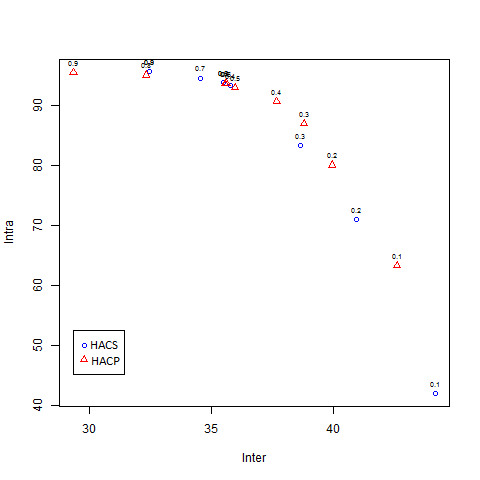
\includegraphics[width=0.50\linewidth]{imagenes/alg1_vs_alg5.png}
	\label{res:inter_intra-1-5}
\end{figure}
}

\frame{\frametitle{Trade-off entre objetivos para los distintos valores de $\gamma$ en $HACS$ y $HACP$}
\begin{itemize}
	\item La mayoría de las soluciones provistas por el algoritmo son no dominadas.
	\item La heurística $HACP+T$ es capaz de proveer conjunto de paquetes con diversos valores de la función $Intra-Inter$.
	\item Incrementos significativos en los valores intra-paquetes no pueden ser alcanzados sin sacrificar el valor inter del conjunto y viceversa.
	\item Este tipo de análisis puede ayudar al usuario a decidirse por una de las soluciones.
	\item Un buen compromiso entre ambas soluciones puede ser la solución $\gamma = 0,3$.
\end{itemize}
}

\section{Conclusiones y trabajo futuro}
\frame{\frametitle{Conclusiones}
\begin{itemize}
	\item La búsqueda y recuperación de la información es una de las aplicaciones más utilizadas en Internet.
	\item En este trabajo se propusieron significativas mejoras a algoritmos para realizar búsquedas de información alternativas a las tradicionales.
	\item Los algoritmos propuestos resultaron más eficientes tanto en valor de la función objetivo como en su sensibilidad al criterio de valoración de cada objetivo, sin perjuicio en el tiempo de ejecución.
\end{itemize}
}

\frame{\frametitle{Trabajo futuro}
\begin{itemize}
	\item Poner algo.
\end{itemize}
}

\end{document}